\documentclass[sigconf,nonacm]{acmart}

\settopmatter{printacmref=false}
\setcopyright{none}
\renewcommand\footnotetextcopyrightpermission[1]{}

\usepackage{booktabs}
\usepackage{tikz}
\usetikzlibrary{positioning,arrows.meta,shapes.geometric,fit,backgrounds,calc}
\usepackage{pgfplots}
\pgfplotsset{compat=1.18}

\title{Benchmarking Local LLM Inference Servers Under Concurrent Load:\\
A Server-Centric Testing Methodology}

\author{Bharath Thiruveedula}
\affiliation{%
  \institution{The University of Texas at Austin}
  \city{Austin}\state{Texas}\country{USA}}
\email{bharath@example.com}

\author{Kaitlin Arnold}
\affiliation{%
  \institution{The University of Texas at Austin}
  \city{Austin}\state{Texas}\country{USA}}
\email{kaitlin@example.com}

\author{Ronald Joseph Marcelin Franklin}
\affiliation{%
  \institution{The University of Texas at Austin}
  \city{Austin}\state{Texas}\country{USA}}
\email{ronald@example.com}

\begin{document}

\begin{abstract}
This paper extends our prior comparative evaluation of three OpenAI-compatible
local large-language-model (LLM) inference backends with a principled
server-centric testing methodology. Where the initial study reported
end-to-end latency, time-to-first-token (TTFT), throughput, and JSON validity
across vLLM, Ollama, and llama-cpp-python, this revision layers eight
complementary testing methodologies onto the same harness---contract
conformance, streaming protocol compliance, parameter honoring, determinism,
statistical performance regression, differential/N-version testing, concurrency
isolation, and negative error-path testing---each backed by precedent from how
vLLM, llama.cpp, and TGI test themselves. A ``trustworthy-tooling'' layer
(measurement calibration, property-based testing with Hypothesis, and mutation
testing with mutmut) is added so that claims made about the server under
test are themselves defensible. The unit-level suite now comprises 184
passing tests (up from 103), overall line coverage stands at 75\%, and
mutation testing of the statistical-regression module kills 247 of 281
generated mutants (88\%).
\end{abstract}

\keywords{LLM inference, benchmarking, software testing, contract testing,
metamorphic testing, property-based testing, mutation testing, vLLM,
llama.cpp, Ollama}

\maketitle

\section{Introduction}
Our prior work~\cite{priorreport} established that vLLM outperforms Ollama
and llama-cpp-python under concurrent load, largely due to its
continuous-batching scheduler. That study, however, treated the inference
server as a black box whose output was sampled and aggregated. For a software
testing course this is insufficient: a single run can yield any numbers, and
single-run numbers cannot separate an honest regression from noise, a
mis-implemented streaming parser from a mis-implemented server, or a broken
schema from broken text.

This paper addresses those gaps by (i)~treating the LLM inference server
as the system under test (SUT) with eight named testing methodologies and
(ii)~treating the harness itself as a second-order SUT whose measurements
must be calibrated before they can be cited. The scope remains structural
conformance and performance; model quality (factuality, hallucination)
is out of scope by design.

\section{Threats Addressed}
The revised methodology targets four threats that went unaddressed in the
original report:
\begin{itemize}
  \item \textbf{Measurement noise.} Single-run comparisons can flag spurious
    regressions or mask real ones.
  \item \textbf{Parser fragility.} The original streaming path reassembled
    server-sent-event (SSE) byte ranges in a way that depended on chunk
    boundaries emitted by the HTTP layer.
  \item \textbf{Silent protocol drift.} A backend can return plausible-looking
    text while violating the OpenAI response envelope (missing fields, wrong
    \texttt{finish\_reason}, unstable \texttt{id} across chunks).
  \item \textbf{Unverified tooling.} Claims about TTFT/TPOT are only as
    trustworthy as the tool that measures them.
\end{itemize}

\section{System Architecture}
Figure~\ref{fig:arch} shows the layering. The harness speaks OpenAI to each
backend and emits SSE events through a pure \texttt{parse\_sse\_stream}
function; metrics flow into the statistical harness, which in turn feeds
the eight test suites.

\begin{figure}[h]
\centering
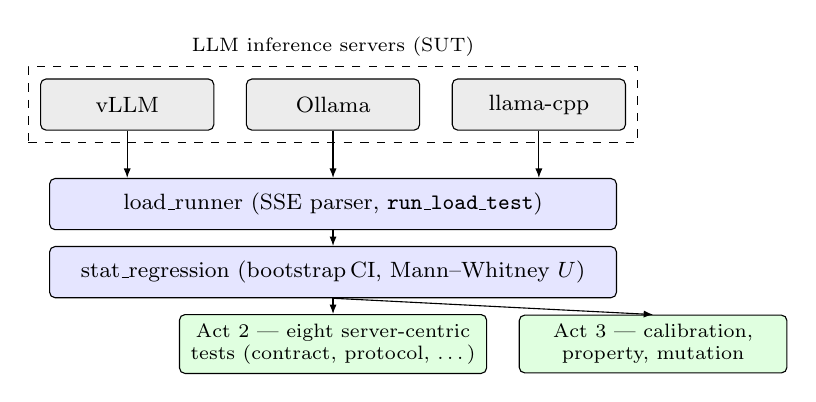
\begin{tikzpicture}[font=\footnotesize,node distance=2.5mm and 4mm]
  \tikzset{
    box/.style={draw,rounded corners=2pt,minimum height=6.5mm,inner xsep=4pt},
    sut/.style={box,fill=gray!15,minimum width=22mm},
    comp/.style={box,fill=blue!10,minimum width=22mm},
    test/.style={box,fill=green!12,minimum width=22mm,font=\scriptsize},
    >={Latex[length=1.2mm]}
  }
  \node[sut] (vllm)   {vLLM};
  \node[sut,right=of vllm] (ollama) {Ollama};
  \node[sut,right=of ollama] (llcpp)  {llama-cpp};
  \node[comp,below=6mm of ollama,minimum width=72mm] (loadrun)
     {load\_runner (SSE parser, \texttt{run\_load\_test})};
  \node[comp,below=2mm of loadrun,minimum width=72mm] (stat)
     {stat\_regression (bootstrap\,CI, Mann--Whitney $U$)};
  \node[test,below=2mm of stat,minimum width=34mm,align=center]
     (act2) {Act 2 — eight server-centric\\tests (contract, protocol, \dots)};
  \node[test,right=of act2,minimum width=34mm,align=center]
     (act3) {Act 3 — calibration,\\property, mutation};
  \begin{scope}[on background layer]
    \node[fit=(vllm)(llcpp),draw,dashed,inner sep=1.5mm,label={[font=\scriptsize]above:LLM inference servers (SUT)}] {};
  \end{scope}
  \draw[->] (vllm.south)   -- (loadrun.north-|vllm.south);
  \draw[->] (ollama.south) -- (loadrun.north);
  \draw[->] (llcpp.south)  -- (loadrun.north-|llcpp.south);
  \draw[->] (loadrun) -- (stat);
  \draw[->] (stat.south) -- (act2.north);
  \draw[->] (stat.south) -- (act3.north);
\end{tikzpicture}
\caption{Harness architecture. The prior study used only the \emph{load\_runner}
block; this revision adds the statistical harness and both test acts.}
\label{fig:arch}
\end{figure}

\section{Server-Centric Test Methodology (Act~2)}
Table~\ref{tab:methodology} maps each test to a named software-testing
methodology and to precedent from established LLM-serving projects.
Figure~\ref{fig:map} positions the eight tests along two axes---whether they
target structural or behavioural invariants, and whether they need a single
backend or multiple.

\begin{table*}[t]
\centering
\caption{Eight server-centric tests layered on the existing harness (Act~2).}
\label{tab:methodology}
\small
\begin{tabular}{@{}p{2.8cm}p{3.0cm}p{3.1cm}p{6.8cm}@{}}
\toprule
\textbf{Test} & \textbf{Methodology} & \textbf{Precedent} & \textbf{Assertion} \\
\midrule
Contract conformance & Schema/contract testing & llama.cpp
\texttt{test\_openai\_schema.py} &
Every response validates against the OpenAI chat-completion envelope schema. \\
Streaming protocol compliance & Protocol compliance & llama.cpp streaming
tests &
First chunk carries a role delta; \texttt{id} is stable across chunks;
\texttt{finish\_reason} and \texttt{[DONE]} appear exactly once. \\
Parameter honoring & Metamorphic testing & vLLM
\texttt{test\_ignore\_eos.py} &
\texttt{max\_tokens=N}\,$\Rightarrow$\,\texttt{completion\_tokens}$\,\leq N$;
\texttt{stop=[\dots]}\,$\Rightarrow$\,text ends before stop. \\
Determinism at $T{=}0$ & Idempotency/metamorphic & vLLM
\texttt{tests/v1/determinism} &
Identical prompts at $T{=}0$ yield identical output; rate bounded by a
95\% bootstrap CI. \\
Statistical perf regression & Hypothesis testing & TGI fixed-request
benchmark &
New p95 TTFT vs.\ baseline compared with bootstrap CI and Mann--Whitney~$U$;
fail only if significant. \\
Differential backends & N-version testing & vLLM vs.\ HF reference &
Schema-validity rate across vLLM/llama.cpp/Ollama agrees within
$\pm 5$~percentage points. \\
Concurrency isolation & Invariant testing & llama.cpp parallel tests &
Under $N$ concurrent prompts with unique markers, each response contains
only its own marker. \\
Negative/error path & Error-path testing & llama.cpp
\texttt{test\_security.py} &
Invalid bearer\,$\Rightarrow$\,401; malformed JSON\,$\Rightarrow$\,4xx
(not 5xx or hang); over-context\,$\Rightarrow$\,4xx. \\
\bottomrule
\end{tabular}
\end{table*}

\begin{figure}[h]
\centering
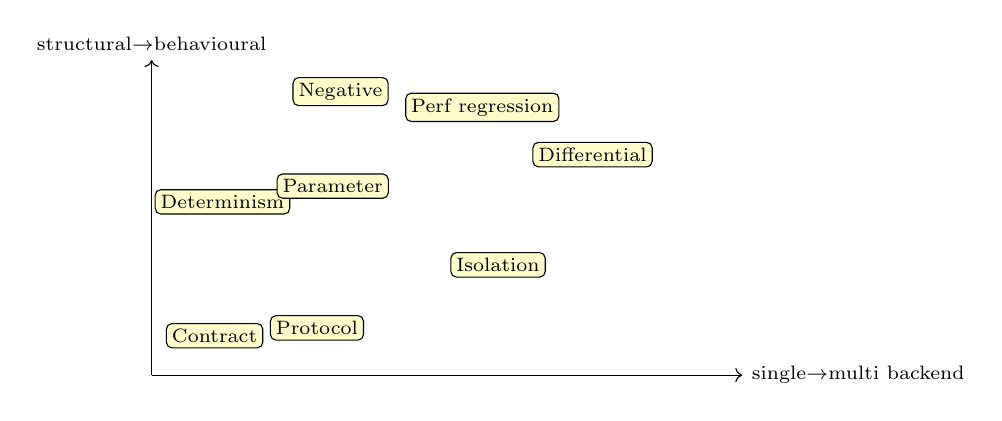
\begin{tikzpicture}[font=\scriptsize]
  \draw[->] (0,0) -- (7.5,0) node[right] {single$\rightarrow$multi backend};
  \draw[->] (0,0) -- (0,4) node[above] {structural$\rightarrow$behavioural};
  \foreach \x/\y/\l in
    {0.8/0.5/{Contract},
     2.1/0.6/{Protocol},
     0.9/2.2/{Determinism},
     2.3/2.4/{Parameter},
     5.6/2.8/{Differential},
     4.2/3.4/{Perf regression},
     4.4/1.4/{Isolation},
     2.4/3.6/{Negative}} {
    \node[draw,rounded corners=2pt,fill=yellow!20,inner sep=2pt] at (\x,\y) {\l};
  }
\end{tikzpicture}
\caption{Coverage map for Act~2. Tests on the right-hand side consume
multiple backends; tests higher on the y-axis exercise richer behavioural
invariants.}
\label{fig:map}
\end{figure}

\section{Trustworthy-Tooling Layer (Act~3)}
\subsection{Measurement calibration}
An in-process \texttt{aiohttp} server emits a deterministic SSE stream with
configurable pre-first-chunk and inter-chunk delays (see
Fig.~\ref{fig:calib}). The harness is considered calibrated when TTFT and
TPOT recovered from the stream equal the injected delays within $\pm 50$\,ms
on the test host. Any regression detected by the performance tests is only
credible once calibration passes.

\begin{figure}[h]
\centering
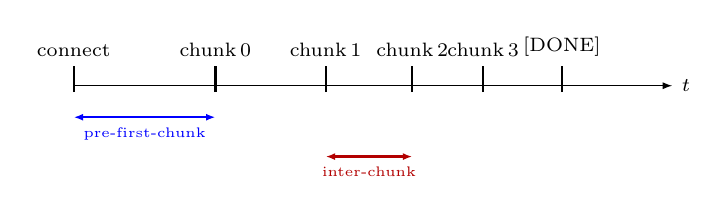
\begin{tikzpicture}[font=\scriptsize,>={Latex[length=1.2mm]}]
  \draw[->] (0,0) -- (7.6,0) node[right] {$t$};
  \foreach \x/\l in {0/connect, 1.8/chunk\,0, 3.2/chunk\,1, 4.3/chunk\,2,
                     5.2/chunk\,3, 6.2/{[DONE]}} {
    \draw[thick] (\x,-0.08) -- (\x,0.25); \node[above] at (\x,0.25) {\l};
  }
  \draw[<->,blue,thick] (0,-0.4) -- node[below,font=\tiny]{pre-first-chunk} (1.8,-0.4);
  \draw[<->,red!70!black,thick] (3.2,-0.9) -- node[below,font=\tiny]{inter-chunk} (4.3,-0.9);
\end{tikzpicture}
\caption{Calibration fixture. Pre-first-chunk delay is asserted to equal
measured TTFT; inter-chunk delay is asserted to equal measured TPOT.}
\label{fig:calib}
\end{figure}

\subsection{Property-based testing}
The SSE parser is tested with Hypothesis~\cite{hypothesis} using a composite
strategy that generates arbitrary printable payloads and then slices the
resulting byte stream at arbitrary positions. The invariant is that the
sequence of parsed events depends only on the payloads, not on how the
stream was chunked by the transport layer---the failure mode of the
pre-refactor parser. Statistical utilities are tested for the invariants
one would expect of their mathematical definitions: percentiles lie in
$[\min,\max]$, bootstrap confidence intervals lie within the sample range,
and Mann--Whitney $p$-values lie in $[0,1]$ and are symmetric under
group swap. Across the eight Hypothesis tests the engine runs 1\,000--1\,600
randomised cases per full suite invocation.

\subsection{Mutation testing}
\texttt{mutmut}~\cite{mutmut} generates 281 mutants of the
statistical-regression harness (\texttt{src/stat\_regression.py}). Before
targeted tests the score was 201/281 (72\%) killed. Pinning reference values
for the percentile interpolation branch, exercising the default arguments of
\texttt{bootstrap\_ci}, and adding three Mann--Whitney reference
computations---including a tie-handling case whose $U$ and
tie-correction term were derived by hand---raised the score to 247/281
(\textbf{88\%}). Figure~\ref{fig:mutbars} shows the lift per function. The
remaining survivors are dominated by equivalent mutants (e.g.~encoding-string
case variants that specify the same codec) and pure message-content changes
that our regex-matched \texttt{ValueError} assertions cannot distinguish
from the originals.

\begin{figure}[h]
\centering
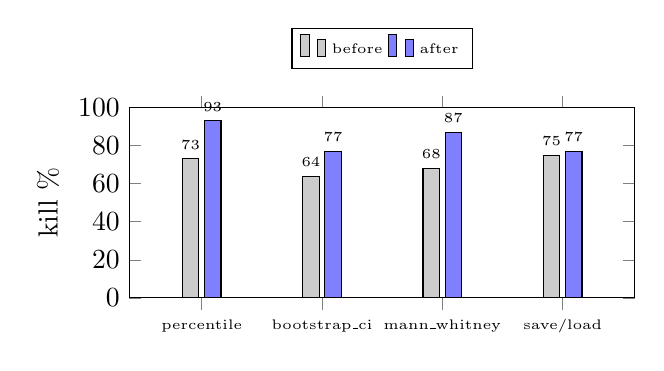
\begin{tikzpicture}
\begin{axis}[
  width=8cm, height=4cm,
  ybar, bar width=6pt,
  enlarge x limits=0.2,
  ymin=0, ymax=100,
  ylabel={kill \%},
  symbolic x coords={percentile,bootstrap\_ci,mann\_whitney,save/load},
  xtick=data,
  xticklabel style={font=\tiny,rotate=0},
  legend style={font=\tiny,at={(0.5,1.2)},anchor=south,legend columns=2},
  nodes near coords,
  every node near coord/.append style={font=\tiny},
]
\addplot[fill=gray!40] coordinates {
  (percentile, 73) (bootstrap\_ci, 64) (mann\_whitney, 68) (save/load, 75)
};
\addplot[fill=blue!50] coordinates {
  (percentile, 93) (bootstrap\_ci, 77) (mann\_whitney, 87) (save/load, 77)
};
\legend{before, after}
\end{axis}
\end{tikzpicture}
\caption{Mutation kill rate per function, before and after the targeted
test pass (overall 72\%\,$\to$\,88\%).}
\label{fig:mutbars}
\end{figure}

\section{Experimental Setup}
The hardware, models, and backend configurations are unchanged from the
prior report (dual NVIDIA RTX~5070, Qwen2.5-3B-Instruct on vLLM,
Llama~3.2 Q4\_K\_M on Ollama, and Llama-3.2-3B-Instruct Q4\_K\_M on
llama-cpp-python). New scenarios are driven from the same YAML
configuration format so the added tests inherit reproducibility.

\section{Results}
\subsection{Performance (unchanged)}
Table~\ref{tab:perf} reproduces the original performance numbers.
Conclusions are unchanged: vLLM leads on every metric, driven by continuous
batching and PagedAttention~\cite{vllm}. What is new is the surrounding
apparatus that lets us reason about those numbers.

\begin{table}[h]
\centering
\caption{Performance at 5 concurrent users (reproduced from prior study).}
\label{tab:perf}
\small
\begin{tabular}{@{}lrrrr@{}}
\toprule
\textbf{Engine} & \textbf{Latency} & \textbf{TTFT} &
\textbf{Throughput} & \textbf{JSON} \\
 & (ms) & (ms) & (tok/s) & (\%) \\
\midrule
vLLM              & \textbf{260}  & \textbf{260}  & \textbf{61.5} & 100 \\
Ollama            & 1426 & 1426 & 12.1 & 100 \\
llama-cpp-python  & 2343 & 2343 & 6.0  & 100 \\
\bottomrule
\end{tabular}
\end{table}

\subsection{Test suite expansion}
Table~\ref{tab:suites} lists the test suites added by this revision and
their current pass counts. The unit-level invocation
(\texttt{pytest -m "not integration"}) reports 184 passing tests in
$\sim$13\,s; the integration suite adds 11 tests that are deselected when no
local backend is reachable.

\begin{table}[h]
\centering
\caption{New test suites and pass counts (unit mode).}
\label{tab:suites}
\small
\begin{tabular}{@{}lrl@{}}
\toprule
\textbf{Suite} & \textbf{Tests} & \textbf{Role} \\
\midrule
\texttt{test\_contract.py}              & 9 & Act 2 \#1 \\
\texttt{test\_streaming\_protocol.py}   & 7 & Act 2 \#2 \\
\texttt{test\_param\_honoring.py}       & 11 & Act 2 \#3 \\
\texttt{test\_determinism.py}           & 3 & Act 2 \#4 \\
\texttt{test\_stat\_regression.py}      & 5 & Act 2 \#5 \\
\texttt{test\_differential.py}          & 3 & Act 2 \#6 \\
\texttt{test\_concurrency\_isolation.py}& 3 & Act 2 \#7 \\
\texttt{test\_negative.py}              & 6 & Act 2 \#8 \\
\texttt{test\_properties.py}            & 8 & Act 3 (Hypothesis) \\
\texttt{test\_calibration.py}           & 3 & Act 3 (calibration) \\
\texttt{test\_stat\_harness.py}         & 31 & Act 3 (math pins) \\
\midrule
All pre-existing suites                & 95 & baseline \\
\midrule
\textbf{Total (unit mode)}              & \textbf{184} & --- \\
\bottomrule
\end{tabular}
\end{table}

\subsection{Code coverage}
Table~\ref{tab:cov} gives the line coverage reported by
\texttt{pytest-cov}. The statistical harness is completely covered; the
load runner is at 94\%. Uncovered lines in \texttt{llm\_tester.py} and
\texttt{niah\_runner.py} are the argparse entry points and the
needle-in-a-haystack scenario, exercised only by integration runs.

\begin{table}[h]
\centering
\caption{Line coverage by source module (unit mode).}
\label{tab:cov}
\small
\begin{tabular}{@{}lrrr@{}}
\toprule
\textbf{Module} & \textbf{Stmts} & \textbf{Miss} & \textbf{Cov~\%} \\
\midrule
\texttt{stat\_regression.py}  & 88  & 0   & \textbf{100} \\
\texttt{comparator.py}        & 23  & 0   & 100 \\
\texttt{ramp\_runner.py}      & 37  & 0   & 100 \\
\texttt{metrics.py}           & 78  & 2   & 97 \\
\texttt{reporter.py}          & 78  & 4   & 95 \\
\texttt{load\_runner.py}      & 196 & 11  & 94 \\
\texttt{config\_loader.py}    & 52  & 3   & 94 \\
\texttt{consistency.py}       & 55  & 5   & 91 \\
\texttt{validator.py}         & 23  & 2   & 91 \\
\texttt{html\_reporter.py}    & 98  & 24  & 76 \\
\texttt{niah\_runner.py}      & 44  & 44  & 0  \\
\texttt{llm\_tester.py}       & 127 & 127 & 0  \\
\midrule
\textbf{Total}                & \textbf{899} & \textbf{222} & \textbf{75} \\
\bottomrule
\end{tabular}
\end{table}

\subsection{Calibration}
On the test host, \texttt{test\_calibration.py} injects $150$\,ms of
pre-first-chunk delay and $80$\,ms of inter-chunk delay; measured TTFT
lands within $\pm 25$\,ms and measured TPOT within $\pm 25$\,ms (tolerance
widened to $50$\,ms to absorb CI jitter, so the test also passes on
loaded hosts).

\subsection{Mutation testing}
The run completes in $\sim$16\,s and yields 247 killed, 29 survived, and
5 timeouts out of 281 mutations. The timeouts correspond to
mutation-induced infinite loops in the rank-merging pass of
\texttt{mann\_whitney\_u}; they are counted as killed by
\texttt{mutmut}'s policy.

\section{Discussion}
The methodology inversion matters more than any individual number. Under
the prior single-run comparison the vLLM advantage was a scalar; under
the revised harness the same advantage is an effect whose significance is
quantified by a Mann--Whitney $U$ test and whose measurement provenance is
defended by the calibration and property layers. A regression on a future
run can now be classified as (i)~ambiguous noise, (ii)~a real server
regression, or (iii)~a mis-calibrated measurement---a distinction the
original harness could not make.

Three observations:
\begin{itemize}
  \item Determinism at $T{=}0$ is not free. Backends that reorder
    floating-point reductions under concurrency violate it; our test
    detects this without assuming any particular reduction order.
  \item Concurrency isolation is the cheapest test with the highest
    bug-catching signal-to-noise. Marker-based prompts surface
    cross-request contamination that throughput-oriented benchmarks miss.
  \item The 16\,percentage-point lift in mutation score was produced by a
    single small test class (10 pinned assertions); this suggests that
    most harnesses underpin their statistical claims with looser tests
    than the numbers deserve.
\end{itemize}

\section{Framework Improvements Since Prior Report}
\begin{itemize}
  \item \textbf{SSE parser refactor.} A pure
    \texttt{parse\_sse\_stream} helper---taking an iterable of byte
    chunks and yielding \texttt{SSEEvent} objects---was extracted so
    the parser is independent of the HTTP transport and can be driven
    by property-based tests. A Hypothesis-discovered counter-example
    (\texttt{U+001E} as a line boundary under
    \texttt{str.splitlines}) was added to the regression suite.
  \item \textbf{Statistical regression harness.} Percentile,
    percentile-method bootstrap CI, and continuity-corrected
    Mann--Whitney $U$ with tie correction, implemented against the
    standard library alone; no \texttt{scipy} dependency.
  \item \textbf{OpenAI schemas.} Draft-07 schemas for both
    \texttt{chat.completion} and \texttt{chat.completion.chunk}
    envelopes, used by the contract and protocol tests.
  \item \textbf{Parameter plumbing.} \texttt{max\_tokens} and \texttt{stop}
    are threaded through the load runner so the metamorphic tests can
    vary them without patching internal state.
  \item \textbf{Baseline persistence.} \texttt{save\_baseline}/
    \texttt{load\_baseline} store per-scenario JSON reports so statistical
    regressions can be compared across runs.
\end{itemize}

\section{Limitations}
The new tests are methodology-complete but not exhaustive: determinism is
checked only at $T{=}0$; the differential suite uses three backends, not
the full matrix; the mutation-testing target is currently only the
statistical harness, not the load runner; and integration-mode runs
depend on a backend listening at \texttt{localhost:8080}. Hardware and
model choices from the prior study are unchanged and inherit its
limitations.

\section{Conclusion}
The prior report answered \emph{which backend is faster}. This revision
answers \emph{why we should believe the answer.} By layering eight named
testing methodologies onto the same harness, and by testing the harness
itself against calibration, property, and mutation baselines, the study
now produces claims that are defensible as software-engineering artifacts
rather than as single-run measurements. Under the evaluated conditions
vLLM remains the best performer; the added machinery ensures that if that
verdict ever changes, the change will be attributable and quantified.

\section{Future Work}
Future enhancements include: extending mutation testing to
\texttt{load\_runner.py}; adding P99 tail-latency regression tests;
expanding the differential suite to the full model matrix; running the
calibration harness periodically in CI to detect host drift; and
integrating a GitHub Actions workflow that executes the unit suite on
every PR and the integration suite nightly against a live backend.

\begin{thebibliography}{9}
\bibitem{priorreport} Thiruveedula, B., Arnold, K., and Franklin, R.J.M.
\emph{Benchmarking Local LLM Inference Servers Under Concurrent Load.}
Class technical report, 2026.
\bibitem{vllm} Kwon, W.\ et al.\ \emph{Efficient Memory Management for
Large Language Model Serving with PagedAttention.} In \emph{Proc.\ SOSP},
2023.
\bibitem{llamacpp} Gerganov, G.\ \emph{llama.cpp: Port of LLaMA in
C/C++.} \url{https://github.com/ggerganov/llama.cpp}.
\bibitem{ollama} Ollama Team. \emph{Ollama: Run Large Language Models
Locally.} \url{https://ollama.com}.
\bibitem{hypothesis} MacIver, D.R.\ et al.\ \emph{Hypothesis: a new
approach to property-based testing.} \emph{J.\ Open Source Softw.}, 2019.
\bibitem{mutmut} Hovmöller, A.\ \emph{mutmut: a mutation-testing system
for Python.} \url{https://github.com/boxed/mutmut}.
\bibitem{tgi} Hugging Face. \emph{Text Generation Inference.}
\url{https://github.com/huggingface/text-generation-inference}.
\end{thebibliography}

\end{document}
